\documentclass{endm}
\usepackage{endmmacro}
\usepackage{graphicx}
\usepackage{longtable}

% The following is enclosed to allow easy detection of differences in
% ascii coding.
% Upper-case    A B C D E F G H I J K L M N O P Q R S T U V W X Y Z
% Lower-case    a b c d e f g h i j k l m n o p q r s t u v w x y z
% Digits        0 1 2 3 4 5 6 7 8 9
% Exclamation   !           Double quote "          Hash (number) #
% Dollar        $           Percent      %          Ampersand     &
% Acute accent  '           Left paren   (          Right paren   )
% Asterisk      *           Plus         +          Comma         ,
% Minus         -           Point        .          Solidus       /
% Colon         :           Semicolon    ;          Less than     <
% Equals        =           Greater than >          Question mark ?
% At            @           Left bracket [          Backslash     \
% Right bracket ]           Circumflex   ^          Underscore    _
% Grave accent  `           Left brace   {          Vertical bar  |
% Right brace   }           Tilde        ~

\newcommand{\Nat}{{\mathbb N}}
\newcommand{\Real}{{\mathbb R}}
\def\lastname{Pinto}

\begin{document}

% DO NOT REMOVE: Creates space for Elsevier logo, ScienceDirect logo
% and ENDM logo
\begin{verbatim}\end{verbatim}\vspace{2.5cm}

\begin{frontmatter}

\title{META-HEURISTICS GRASP AND ILS APPLIED TO THE AIRCRAFT ROTATION PROBLEM}

\author{Alexander de Almeida Pinto}
\address{LAVID\\ Federal University of Paraiba \\ Joao Pessoa, Brazil}

\author{Daniel Goncalvez Ramos}
\address{LAVID\\ Federal University of Paraiba \\ Joao Pessoa, Brazil}

\author{Lucidio dos Anjos Formiga Cabral}
\address{IT Department\\ Federal University of Paraiba \\ Joao Pessoa, Brazil}

\begin{abstract}
The Aircraft Rotation Problem refers to the designation of each airplane available at airlines companies such that all planned flights are covered. This is a light constrained problem since any aircraft can be assigned to an unlimited quantity of duty work. However, there are many lower cost solutions that can be obtained by simply adjusting the time of departure of a flight, or even positioning some aircraft by executing ferry flights between two near airports. We describe an algorithm based on GRASP meta-heuristic using ILS as local search, which calculates a sub-optimal way to organize the flights. This is a good solution to large scaled problems, considering that in this case, an exact method would require some years to be applied. Some computational results are presented for a real world problem at Rio-Sul Brazilian Airline.
\end{abstract}

\begin{keyword}
Aircraft Routing, Optimization, Meta-heuristic, GRASP
\end{keyword}

\end{frontmatter}


\section{Introduction}\label{intro}

The airline industry has been a rich source of problems related to operational research, mainly due to combinatorial explosive nature of these problems. Typically, planning problems involve the creation of lines of work for both aircraft and crew.

On the literature, there are two well-known problems associated to aircraft planning, the Fleet Assignment and the Aircraft Rotation Problem (ARP). The first deals with the allocation of the fleet, determining the type of aircraft used in each flight \cite{pimentel2005}. The second is the one covered on this paper, and will be explained on the next section.

Due to the combinatorial explosion of the problems involving airlines, they should be solved separately, though each problem should be solved giving conditions to the next one be solved. 

Many techniques have been used to give a solution to the ARP, some of them using exact methods, which always obtain the best result, but uses lots of CPU, and in practice is unfeasible, due to the size of real problems. Other techniques try to find a good solution, instead of the best, and try to do that in a fast way. To do so, they use meta-heuristics, a heuristic method that uses some historical knowledge of the solutions combined with some characteristic of the problem to find a good solution for big instances.

\subsection{The ARP problem}

After solving the Fleet Assignment problem, the one that chooses the kind of airplane that will cover the flights, the problem becomes the organization of the flights. It means, how flights will be connected. The ways to group them can have a very big impact on the cost of the flight network. This cost comes from several factors, like the numbers of aircrafts needed to cover all the flights, the delay between them, the downtime of the flights, and others.

To solve this problem, we must be aware of some constraints involving time and space. For example, an airplane cannot leave before the arrival of the flight that precedes it, neither from a different city that it has arrived on the last flight. Though these are obvious constraints, they make the problem really hard to solve in a large scale, as we could have a very big number of combinations between the connections of the flights. There is also another constraint, related to the time that the airplane has to be on the ground before it leaves. This restriction is usually related to an airport.

Considering these restrictions, we should arrange the flights looking for a cheap network. Its known that finding the cheapest is almost impossible for big instances, but finding a good one can be achieved with some meta-heuristics.

	Another important aspect is the maintaining restrictions. It is known that a plane must have periodic checks. Opportunities to perform these tasks occur only on some connections that are potentially available. As consequence, a sequence of flights must be constructed so that these restrictions are not violated. In order to easily incorporate these constraints in our framework, we assume that the rotations are not assigned to specific types of aircraft. Thus, if an aircraft needs maintenance, is created a special flight depart and arrive from the maintenance base chosen. The time of flight is exactly the service time \cite{pimentel2005}.

\section{Methodology}

In order to find a good solution to the ARP problem, two meta-heuristics were implemented using java Language. On this section, it will be exposed how to represent a solution, as well as some details about the application of the meta-heuristics on the ARP problem.

\subsection{Problem Concepts}

Each solution has the flight network, with all the connections between the flights. To represent the flights covered by a unique airplane, the concept of a track was applied. So, the goal is to find the smallest number of tracks needed to cover all flights.

	Each track is composed by any number of flights, considering the restrictions described on last section. The connection between flights is called arc. An arc has to be one of the followings:

\begin{itemize}

\item Simple Connection Arc (type 1): This arc connects flights that don’t need to be changed. There is no need to create another flight to connect them too. The cost of this arc is zero.

\item Connection With Delay Arc (type 2): With this arc, the second flight needs to be delayed, in order to conform the time restriction. The cost of this arc is the delay (in minutes) of the second flight.

\item Connection With Repositioning Arc (type 3): This arc creates a third flight between the two previously selected, in order to conform the space condition. The third flight goes from the destination of the first flight to the origin of the second flight. The cost of this arc is the duration of the created flight.

\item Connection With Repositioning and Delay Arc (type 4): Besides creating a new flight to connect the two ones, this type of arc also delays the second flight, so it obeys both space and time restrictions. The cost of this arc is the addition of the delayed time plus the duration of the created flight.
\end{itemize}

\subsection{Problem Solution and Representation}

The generation of a solution was divided into two steps. The first one constructs a good solution and the second tries to improve the given solution with some local search algorithms.

To generate a solution, the algorithm GRASP (Greedy Randomized Adaptive Search Procedure) was applied. This algorithm utilizes a greedy heuristic, mixed with a nondeterministic choice of the next element to the solution [FONTE]. To do so, each time an element is to be added to the solution, it is chosen randomically between a fraction of the best ones, according to a greedy algorithm. The algorithm runs several times, and only the best solution goes to the next step.

The second meta-heuristic applied to the ARP is the Iterated Local Search (ILS). It takes a given solution, found on the first phase, and makes some search on different neiborghoods. With this, local minimums can be avoided [Fonte].

It was developed a visual interface to show the solution found by the algorithms. It can be viewed in the results section, picture 1.

\section{The constructive algorithm}

In this phase, the computer generates a good solution, following the steps:

\subsection{Track formation}
\subsubsection{ Initializing a track }

To initialize a track, a flight is randomically chosen between the N flights that have the lower departure time and that have not been chosen by another track.

\subsubsection{ Composing and finalizing a track }

After choosing the first flight, or with the previous flight, it is made the choice of the next arch k,  $ K \in \{ 1, 2, 3, 4 \} $. This choice is made with a probability associated with each arch type P1, P2, P3, P4. The next flight should obey the arch rule and should not have a departure time very far from the arrival of the last. With all the candidates, only the a\% best are chosen to be a part of the possible set. So it is randomically picked one and added to the track.

The value of ‘a’ was defined as 15\%, to type 1 arches, and variable, according to the number of candidates, to the other arches.

If the generated set don’t have any flight, then the arch type will be changed. If no arch have any possible flight, then the last flight ends the track.

\subsection{ Composing a network }

It is generated as much tracks as all the flights are covered. The constructive algorithm stops when all the flights are already corered.	

\section{The local search Algorithm}

After selecting the best solution generated in construction, it is used some algorithms to try to find a way to improve the solution. It was used the swap and compaction methods and the ILS (Iterated Local Search) meta-heuristic.

There were three kinds of swaps implemented, the Swap-1, Swap-2 and the Swap 3. The swap-n procedure is done by trying to change n connected flights with 1 to n + 1 flights. The change is accepted if there is a cost reduction. The compaction method tries to merge two different tracks into one. 

The ILS algorithm was implemented in a way of disturbing the current solution, and then applying the methods described before. Forcing four Swaps-2, not considering if they improve the solution, makes this disturbance.


\subsection{Computational results}

To run the tests, it was used a small daily flight network from Rio-Sul airlines \cite{pimentel2005}. All data is described on Appendix A to D. With this information, any program can be tested with the same entrance, verifying its efficiency. 

All tests run on a Intel Core 2 T5300 1.73GHz, with 1GB DDR-2 RAM. The algorithm was implemented using Java, on NetBeans IDE 6.0.1.

The table below shows details of the achievement of the best solution:\\


\begin{center}

\label {tabela1}
\begin{tabular}{ccc} 

\hline

Number of tracks & Cost & Time(seconds) \\ 

\hline
\hline
21 & 21335 & 0.039 \\
17 & 17100 & 0.113 \\
17 & 17078 & 0.315 \\
17 & 17074 & 0.346 \\
17 & 17066 & 6.012 \\
17 & 17054 & 9.612 \\
17 & 17048 & 14.179 \\
17 & 17040 & 15.0 \\
17 & 17033 & 19.484 \\
\hline
&  & \\
\end{tabular}

\end{center}

Below we have a visualization of the best result obtained:

%\begin{center}
%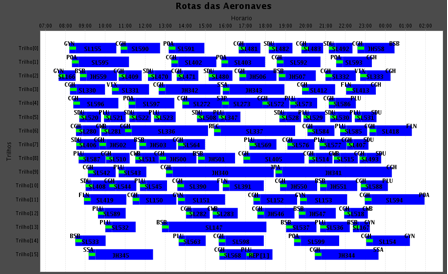
\includegraphics[]{img/formacao.png}
%\end{center}

This result can be viewed in more detail in Attachment C.

In the test described was set a ground time standard for all airports, which is 20 minutes. The time between two airports can be found in Attachment B

\subsection{Conclusion and Future Researches}

The aircrafts are one of the most expensive resources on aeronautics, so every flight planning should be done for a cost reduction. The ARP is one of the problems that can lead to a very high operational cost to a company, if erroneously treated or ignored.

With simple time changing or creating a repositioning flight, the flight network could have a substantial improvement, decreasing aircrafts downtime and reducing the number of planes needed to cover all the defined flights.

For next researches, some efforts are being made to idealize a more complete model of the ARP, leading with weekly tasks, and also solve the next problem to the ARP, the Crew Scheduling. On this next approach, not only the flights will be organized, but also all the crew will be designated to cover the network.

\begin{thebibliography}{10}\label{bibliography}

\bibitem{pimentel2005} Pimentel, A. G., \emph{Uma abordagem heur\'istica para a solu\c{c}\~ao de problemas de recobrimento de conjuntos de grande porte, com aplica\c{c}\~ao \`a aloca\c{c}\~ao de tripula\c{c}\~oes para companhias a\'ereas}, Tese de Doutorado, Universidade Federal do Rio de Janeiro (2002).

\bibitem{pontes2002} Pontes, R., Lucena, A. e Cabral, L., \emph{Exact and Heuristic Techniques for Solving the Aircraft
Rotation Problem}, Technical report Department of Statistics UFPB (2002).

\bibitem{rezende1998} Rezende, M, \emph{Greedy Randomized Adaptative Search Procedures (GRASP) }, Technical 
Report, ATT Labs Research (1998).
  
 \bibitem{rubin1973} Rubin, J. , ``A Technique for the Solution of Massive Set Covering Problems with Application 
to Airline Crew Scheduling,'' Transportation Science (1973).
  
 \bibitem{clarke1997} Clarke L, Johnson E, Nemhauser G, Zhu ZX, ``The Aircraft Rotation Problem,'' Annals of 
Operations Research (1997) 69: 33-46
  
\bibitem{klabjan1999} Klabjan, D. Johnson, E. Nemhauser, G., ``Solving Large Airline Crew Scheduling 
Problems: Random Pairing Generation and Strong Branching,'' Technical Report, Georgia Institute of 
Technology (1999).  

\end{thebibliography}



\appendix

\newpage
\section{Flights Network}

\begin{center}


\renewcommand{\arraystretch}{0.6}

\label {tabela1}
\begin{longtable}{lll} 


  \scriptsize001 SL166 08:00 08:31 GYN BSB  & \scriptsize  037 JH500 13:02 14:33 CGH BSB & \scriptsize 073 JH550 19:04 20:35 CGH BSB\\
  \scriptsize002 SL155 08:32 10:33 GYN CGH  &  \scriptsize  038 SL147 13:10 18:03 BSB BSB   & \scriptsize074 SL537 19:22 20:33 BSB PLU\\
  \scriptsize003 SL330 08:34 09:59 CGH VIX    &  \scriptsize  039 JH340 13:22 18:25 CGH JPA   &  \scriptsize 075 SL576 19:26 20:27 CGH PLU \\
  \scriptsize004 SL595 08:40 11:11 POA CGH    &  \scriptsize  040 SL591 13:30 14:57 POA CGH &  \scriptsize076 SL573 19:34 20:35 PLU CGH  \\
  \scriptsize005 SL596 08:44 10:39 CGH POA  &  \scriptsize  041 SL402 13:38 15:33 CGH POA     &  \scriptsize 077 SL599 19:46 21:41 POA CGH  \\
  \scriptsize006 SL533 08:50 10:01 BSB PLU   &   \scriptsize  042 SL471 13:54 14:39 CGH SDU  & \scriptsize 078 JH547 20:00 21:31 BSB CGH\\
  \scriptsize007 SL280 08:52 09:43 CGH CWB  &  \scriptsize  043 SL390 13:56 15:41 CGH FLN   &  \scriptsize  079 SL153 20:04 22:05 GYN CGH\\
  \scriptsize008 SL587 09:00 10:01 PLU CGH    &  \scriptsize  044 SL564 13:58 14:59 CGH PLU  &  \scriptsize   080 SL483 20:08 20:53 CGH SDU \\
  \scriptsize009 SL520 09:02 09:47 SDU PLU   & \scriptsize  045 SL151 13:58 15:59 GYN CGH   &  \scriptsize   081 SL412 20:10 21:29 CGH FLN \\
  \scriptsize010 JH559 09:04 10:35 BSB CGH   &  \scriptsize  046 SL563 14:00 15:01 PLU CGH    & \scriptsize  082 SL529 20:14 20:59 PLU SDU \\
  \scriptsize011 SL406 09:06 09:55 SDU CGH &    \scriptsize 047 SL272 14:12 15:51 CGH SJP   &    \scriptsize 083 SL584 20:26 21:27 CGH PLU\\
  \scriptsize012 SL419 09:16 11:03 FLN CGH   &  \scriptsize  048 SL282 14:22 15:13 CGH CWB  &  \scriptsize  084 SL514 20:30 21:21 CGH CWB \\
  \scriptsize013 SL542 09:28 10:31 CGH PLU    &  \scriptsize  049 SL508 14:56 15:41 SDU PLU   &  \scriptsize   085 JH344 20:48 23:39 CGH SSA \\
  \scriptsize014 SL408 09:30 10:21 SDU CGH    & \scriptsize  050 JH501 14:58 16:29 BSB CGH   &  \scriptsize  086 SL577 21:02 22:03 PLU CGH   \\
  \scriptsize015 JH345 09:30 12:23 SSA CGH   & \scriptsize  051 SL480 15:30 16:21 SDU CGH   &   \scriptsize  087 SL536 21:04 22:13 PLU BSB  \\
  \scriptsize016 SL589 09:58 11:01 PLU CGH    & \scriptsize  052 SL283 15:42 16:37 CWB CGH  &  \scriptsize   088 JH551 21:04 22:35 BSB CGH  \\
  \scriptsize017 JH502 10:02 11:33 CGH BSB   & \scriptsize  053 SL337 15:46 19:29 REC CGH    &  \scriptsize  089 SL332 21:20 22:31 CGH VIX  \\
  \scriptsize018 SL281 10:08 10:59 CWB CGH & \scriptsize  054 SL347 16:00 16:45 PLU SDU    &    \scriptsize  090 SL492 21:30 22:21 SDU CGH\\
  \scriptsize019 SL521 10:16 11:01 PLU SDU  & \scriptsize 055 SL598  16:00 17:55 CGH POA    &    \scriptsize  091 SL586 21:30 22:31 CGH PLU\\
  \scriptsize020 SL532 10:20 11:31 PLU BSB   & \scriptsize056 SL568 16:02 17:03 CGH PLU  &    \scriptsize 092 SL530 21:34 22:19 SDU PLU\\
  \scriptsize021 SL510 10:22 11:13 CGH CWB & \scriptsize057 SL403 16:08 17:59 POA CGH   &  \scriptsize  093 SL515 21:45 22:37 CWB CGH\\
  \scriptsize022 SL544 10:32 11:33 CGH PLU & \scriptsize058 SL273 16:10 17:51 SJP CGH   &   \scriptsize  094 SL593 21:52 23:19 POA CGH \\
  \scriptsize023 SL331 10:40 12:11 VIX CGH   & \scriptsize059 SL391 16:12 17:55 FLN CGH  &  \scriptsize  095 SL585 22:04 23:05 PLU CGH  \\
 \scriptsize 024 SL409 11:00 11:49 CGH SDU  & \scriptsize 060 JH343 16:12 18:57 SSA CGH &  \scriptsize 096 SL518 22:16 23:07 CGH CWB    \\
 \scriptsize 025 SL543 11:00 12:03 PLU CGH & \scriptsize 061 SL481 17:00 17:45 CGH SDU   &   \scriptsize  097 SL413 22:22 23:31 FLN CGH \\
 \scriptsize 026 SL590 11:06 12:44 CGH POA  & \scriptsize 062 JH506 17:02 18:33 CGH BSB &   \scriptsize  098 SL407 22:24 23:09 CGH SDU \\
 \scriptsize 027 SL336 11:16 15:05 CGH REC  & \scriptsize063 SL405 17:14 19:57 CGH CGH   &   \scriptsize   099 SL167 22:42 23:13 BSB GYN\\
 \scriptsize 028 SL597 11:30 13:27 POA CGH   &  \scriptsize 064 SL569 17:32 18:33 PLU CGH  &   \scriptsize  100 SL531 22:48 23:33 PLU SDU \\
\scriptsize  029 SL522 11:32 12:17 SDU PLU   & \scriptsize 065 SL152 17:44 19:35 CGH GYN   &   \scriptsize 101 JH558 22:56 00:27 CGH BSB\\
\scriptsize  030 SL150 11:42 13:33 CGH GYN  & \scriptsize066 JH546 17:56 19:27 CGH BSB   &   \scriptsize   102 SL493 23:02 23:47 CGH SDU\\
\scriptsize  031 SL511 11:50 12:41 CWB CGH  & \scriptsize067 SL572 17:58 18:59 CGH PLU  &   \scriptsize  103 SL333 23:04 00:15 VIX CGH\\
\scriptsize  032 JH503 12:02 13:33 BSB CGH    & \scriptsize068 SL482 18:30 19:21 SDU CGH &  \scriptsize  104 SL588 23:06 00:07 CGH PLU\\
\scriptsize  033 SL545 12:04 13:05 PLU CGH   & \scriptsize069 JH341 18:50 00:19 JPA CGH  &   \scriptsize   105 SL594 23:18 01:57 CGH POA\\
\scriptsize  034 SL470 12:28 13:19 SDU CGH  & \scriptsize070 SL592 18:54 20:45 CGH POA  &  \scriptsize   106 SL154 23:22 01:13 CGH GYN \\
\scriptsize  035 SL523 12:46 13:31 PLU SDU   & \scriptsize071 JH507 19:00 20:31 BSB CGH  &   \scriptsize   107 SL418 23:32 01:19 CGH FLN\\
\scriptsize  036 JH342 13:00 15:45 CGH SSA & \scriptsize 072 SL528 19:02 19:47 SDU PLU & \\

\end{longtable}

\end{center}

\newpage
\section{Flight Time Between Airports}

\begin{center}

\renewcommand{\arraystretch}{0.6}

\label {tabela2}
\begin{longtable}{llll} 

\scriptsize BSB – CGH  091 & \scriptsize BSB – CWB  125 & \scriptsize BSB – FLN  152 & \scriptsize BSB – GYN  031\\
\scriptsize BSB – JPA  197 & \scriptsize BSB – PLU  071 & \scriptsize BSB – POA  185 & \scriptsize BSB – REC  191\\
\scriptsize BSB – SDU  107 & \scriptsize BSB – SJP  066 & \scriptsize BSB – SSA  125 & \scriptsize BSB – VIX  109\\
\scriptsize CGH – CWB  051 & \scriptsize CGH – FLN  105 & \scriptsize CGH – GYN  095 & \scriptsize CGH – JPA  255\\
\scriptsize CGH – PLU  058 & \scriptsize CGH – POA  097 & \scriptsize CGH – REC  246 & \scriptsize CGH – SDU  049\\
\scriptsize CGH – SJP  049 & \scriptsize CGH – SSA  171 & \scriptsize CGH – VIX  087 & \scriptsize CWB – FLN  028\\	
\scriptsize CWB – GYN  114 & \scriptsize CWB – JPA  293 & \scriptsize CWB – PLU  095 & \scriptsize CWB – POA  062\\
\scriptsize CWB – REC  283 & \scriptsize CWB – SDU  078 & \scriptsize CWB – SJP  060 & \scriptsize CWB – SSA  208\\	
\scriptsize CWB – VIX  125 & \scriptsize FLN – GYN  142 & \scriptsize FLN – JPA  311 & \scriptsize FLN – PLU  114\\	
\scriptsize FLN – POA  042 & \scriptsize FLN – REC  300 & \scriptsize FLN – SDU  087 & \scriptsize FLN – SJP  088\\	
\scriptsize FLN – SSA  225 & \scriptsize FLN – VIX  136 & \scriptsize GYN – JPA  216 & \scriptsize GYN – PLU  076	\\
\scriptsize GYN – POA  173 & \scriptsize GYN – REC  210 & \scriptsize GYN – SDU  109 & \scriptsize GYN – SJP  054\\	
\scriptsize GYN – SSA  143 & \scriptsize GYN – VIX  118 & \scriptsize JPA – PLU  198 & \scriptsize JPA – POA  352\\	
\scriptsize JPA – REC  013 & \scriptsize JPA – SDU  226 & \scriptsize JPA – SJP  251 & \scriptsize JPA – SSA  085	\\
\scriptsize JPA – VIX  181	 & \scriptsize PLU – POA  155 & \scriptsize PLU – REC  187 & \scriptsize PLU – SDU  045	\\
\scriptsize PLU – SJP  067 & \scriptsize PLU – SSA  113 & \scriptsize PLU – VIX  044 & \scriptsize POA – REC  342	\\
\scriptsize POA – SDU  129 & \scriptsize POA – SJP  119 & \scriptsize POA – SSA  267 & \scriptsize POA – VIX  177\\	
\scriptsize REC – SDU  215 & \scriptsize REC – SJP  242 & \scriptsize REC – SSA  075 & \scriptsize REC – VIX  169\\	
\scriptsize SDU – SJP  079 & \scriptsize SDU – SSA  130 & \scriptsize SDU – VIX  048 & \scriptsize SJP – SSA  169\\	
\scriptsize SJP – VIX  110 & \scriptsize 	SSA – VIX  097 & & \\


\end{longtable}

\end{center}

\newpage
\section{Result Obtained By The GRASP}

\begin{center}

\renewcommand{\arraystretch}{0.6}

\label {tabela3}
\begin{longtable}{lll} 

\\

\scriptsize Trilho[1] &	 \scriptsize Trilho[2] & \scriptsize Trilho[3]\\
\scriptsize SL155 08:32 10:33 GYN CGH  & \scriptsize SL595 08:40 11:11 POA CGH & 		\scriptsize SL166 08:00 08:31 GYN BSB\\
\scriptsize SL590 11:06 12:44 CGH POA	 & \scriptsize SL402 13:38 15:33 CGH POA &		\scriptsize JH559 09:04 10:35 BSB CGH\\
\scriptsize SL591 13:30 14:57 POA CGH & 	\scriptsize SL403 16:08 17:59 POA CGH & 	\scriptsize SL409 11:00 11:49 CGH SDU\\
\scriptsize SL481 17:00 17:45 CGH SDU & 	\scriptsize SL592 18:54 20:45 CGH POA & 	\scriptsize SL470 12:28 13:19 SDU CGH\\
\scriptsize SL482 18:30 19:21 SDU CGH & 	\scriptsize SL593 21:52 23:19 POA CGH & 	\scriptsize SL471 13:54 14:39 CGH SDU\\
\scriptsize SL483 20:08 20:53 CGH SDU & 	\scriptsize SL480 15:30 16:21 SDU CGH  & \\
\scriptsize SL492 21:30 22:21 SDU CGH & 	\scriptsize JH506 17:02 18:33 CGH BSB  & \\
\scriptsize JH558 22:56 00:27 CGH BSB &       \scriptsize JH507 19:00 20:31 BSB CGH  & \\
\scriptsize SL332 21:20 22:31 CGH VIX  &  & \\
\scriptsize SL333 23:04 00:15 VIX CGH   &    & \\ 
	
\\
\scriptsize Trilho[4] &       \scriptsize Trilho[5] &       \scriptsize Trilho[6] \\
\scriptsize SL330 08:34 09:59 CGH VIX &       \scriptsize SL596 08:44 10:39 CGH POA &       \scriptsize SL520 09:02 09:47 SDU PLU \\
\scriptsize SL331 10:40 12:11 VIX CGH &       \scriptsize SL597 11:30 13:27 POA CGH &       \scriptsize SL521 10:16 11:01 PLU SDU\\
\scriptsize JH342 13:00 15:45 CGH SSA &       \scriptsize SL272 14:12 15:51 CGH SJP (-1) &       \scriptsize SL522 11:32 12:17 SDU PLU\\
\scriptsize JH343 16:12 18:57 SSA CGH &       \scriptsize SL273 16:10 17:51 SJP CGH &       \scriptsize SL523 12:46 13:31 PLU SDU\\
\scriptsize SL412 20:10 21:29 CGH FLN &       \scriptsize SL572 17:58 18:59 CGH PLU (+13) &       \scriptsize SL508 14:56 15:41 SDU PLU (-1)\\
\scriptsize SL413 22:22 23:31 FLN CGH &       \scriptsize SL573 19:34 20:35 PLU CGH &       \scriptsize SL347 16:00 16:45 PLU SDU\\
\scriptsize SL586 21:30 22:31 CGH PLU &       \scriptsize SL528 19:02 19:47 SDU PLU & \\
\scriptsize SL529 20:14 20:59 PLU SDU & & \\
\scriptsize SL530 21:34 22:19 SDU PLU & & \\
\scriptsize SL531 22:48 23:33 PLU SDU & & \\

\\

\scriptsize Trilho[7] &       \scriptsize Trilho[8] &       \scriptsize Trilho[9] \\
\scriptsize SL280 08:52 09:43 CGH CWB &       \scriptsize SL406 09:06 09:55 SDU CGH (-13) &       \scriptsize SL587 09:00 10:01 PLU CGH\\
\scriptsize SL281 10:08 10:59 CWB CGH &       \scriptsize JH502 10:02 11:33 CGH BSB	 &       \scriptsize SL510 10:22 11:13 CGH CWB\\
\scriptsize SL336 11:16 15:05 CGH REC (+3) &       \scriptsize JH503 12:02 13:33 BSB CGH &       \scriptsize SL511 11:50 12:41 CWB CGH\\
\scriptsize SL337 15:46 19:29 REC CGH &       \scriptsize SL564 13:58 14:59 CGH PLU &       \scriptsize JH500 13:02 14:33 CGH BSB\\
\scriptsize SL584 20:26 21:27 CGH PLU &       \scriptsize SL569 17:32 18:33 PLU CGH &       \scriptsize JH501 14:58 16:29 BSB CGH\\
\scriptsize SL585 22:04 23:05 PLU CGH &       \scriptsize SL576 19:26 20:27 CGH PLU &       \scriptsize SL405 17:14 19:57 CGH CGH\\
\scriptsize SL418 23:32 01:19 CGH FLN &       \scriptsize SL577 21:02 22:03 PLU CGH &       \scriptsize SL514 20:30 21:21 CGH CWB \\
\scriptsize SL407 22:24 23:09 CGH SDU &       \scriptsize SL515 21:45 22:37 CWB CGH  &   \\
\scriptsize SL493 23:02 23:47 CGH SDU &   &   \\

\\

\scriptsize Trilho[10] &       \scriptsize Trilho[11] &       \scriptsize Trilho[12] \\
\scriptsize SL542 09:28 10:31 CGH PLU &       \scriptsize SL408 09:30 10:21 SDU CGH (-9) &       \scriptsize SL419 09:16 11:03 FLN CGH\\
\scriptsize SL543 11:00 12:03 PLU CGH &       \scriptsize SL544 10:32 11:33 CGH PLU &       \scriptsize SL150 11:42 13:33 CGH GYN\\
\scriptsize JH340 13:22 18:25 CGH JPA &       \scriptsize SL545 12:04 13:05 PLU CGH &       \scriptsize SL151 13:58 15:59 GYN CGH\\
\scriptsize JH341 18:50 00:19 JPA CGH &       \scriptsize SL390 13:56 15:41 CGH FLN &       \scriptsize SL152 17:44 19:35 CGH GYN\\
\scriptsize SL391 16:12 17:55 FLN CGH &       \scriptsize SL153 20:04 22:05 GYN CGH & \\
\scriptsize JH550 19:04 20:35 CGH BSB &       \scriptsize SL594 23:18 01:57 CGH POA & \\
\scriptsize JH551 21:04 22:35 BSB CGH	& & \\
\scriptsize SL588 23:06 00:07 CGH PLU	& & \\

\\

\scriptsize Trilho[13] &       \scriptsize Trilho[14] &       \scriptsize Trilho[15] \\
\scriptsize SL589 09:58 11:01 PLU CGH &       \scriptsize SL532 10:20 11:31 PLU BSB &       \scriptsize SL533 08:50 10:01 BSB PLU \\
\scriptsize SL282 14:22 15:13 CGH CWB &       \scriptsize 	SL147 13:10 18:03 BSB BSB &       \scriptsize SL563 14:00 15:01 PLU CGH \\
\scriptsize SL283 15:42 16:37 CWB CGH &       \scriptsize 	SL537 19:22 20:33 BSB PLU &       \scriptsize SL598 16:00 17:55 CGH POA \\
\scriptsize JH546 17:56 19:27 CGH BSB &       \scriptsize SL536 21:04 22:13 PLU BSB &       \scriptsize SL599 19:46 21:41 POA CGH \\
\scriptsize JH547 20:00 21:31 BSB CGH &       \scriptsize SL167 22:42 23:13 BSB GYN &       \scriptsize SL154 23:22 01:13 CGH GYN \\
\scriptsize SL518 22:16 23:07 CGH CWB	 & & \\	

\\
		
\scriptsize Trilho[16]	& & \\	
\scriptsize JH345 09:30 12:23 SSA CGH	& & \\
\scriptsize SL568 16:02 17:03 CGH PLU	& & \\
\scriptsize NOVO  17:23 18:21 PLU CGH	& & \\
\scriptsize JH344 20:48 23:39 CGH SSA	& & \\	


		
\end{longtable}

\end{center}

\newpage
\section{Colision with window}

All ground time is fixed in 20 minutes.

\begin{center}

\renewcommand{\arraystretch}{0.6}

\label {tabela4}
\begin{longtable}{lll} 

\hline
\scriptsize 16 Flights with up to 1 minute window & \scriptsize 15 Flights with up to 17 minute window & \scriptsize 14 Flights with up to 33 minute window \\
\hline
\\

\scriptsize 001 SL155 0 08:32 0 10:33 GYN CGH & \scriptsize 068 JH341 0 18:50 1 00:19 JPA CGH & \scriptsize 001 SL155 0 08:32 0 10:33 GYN CGH\\
\scriptsize 002 SL330 0 08:34 0 09:59 CGH VIX & \scriptsize 069 SL592 0 18:54 0 20:45 CGH POA & \scriptsize 002 SL330 0 08:34 0 09:59 CGH VIX\\
\scriptsize 003 SL595 0 08:40 0 11:11 POA CGH & \scriptsize 070 JH507 0 19:00 0 20:31 BSB CGH & \scriptsize 003 SL595 0 08:40 0 11:11 POA CGH\\
\scriptsize 004 SL596 0 08:44 0 10:39 CGH POA & \scriptsize 072 JH550 0 19:04 0 20:35 CGH BSB & \scriptsize 004 SL596 0 08:44 0 10:39 CGH POA\\
\scriptsize 005 SL533 0 08:50 0 10:01 BSB PLU & \scriptsize 073 SL537 0 19:22 0 20:33 BSB PLU & \scriptsize 	005 SL533 0 08:50 0 10:01 BSB PLU\\
\scriptsize 006 SL280 0 08:52 0 09:43 CGH CWB & \scriptsize 074 SL576 0 19:26 0 20:27 CGH PLU & \scriptsize 006 SL280 0 08:52 0 09:43 CGH CWB\\
\scriptsize 007 SL587 0 09:00 0 10:01 PLU CGH & \scriptsize 075 SL573 0 19:34 0 20:35 PLU CGH & \scriptsize 007 SL587 0 09:00 0 10:01 PLU CGH\\
\scriptsize 008 SL520 0 09:02 0 09:47 SDU PLU & \scriptsize 076 SL599 0 19:46 0 21:41 POA CGH & \scriptsize 008 SL520 0 09:02 0 09:47 SDU PLU\\
\scriptsize 009 JH559 0 09:04 0 10:35 BSB CGH & \scriptsize 077 JH547 0 20:00 0 21:31 BSB CGH & \scriptsize 009 JH559 0 09:04 0 10:35 BSB CGH\\
\scriptsize 010 SL406 0 09:06 0 09:55 SDU CGH & \scriptsize 078 SL153 0 20:04 0 22:05 GYN CGH & \scriptsize 010 SL406 0 09:06 0 09:55 SDU CGH\\
\scriptsize 011 SL419 0 09:16 0 11:03 FLN CGH & \scriptsize 079 SL483 0 20:08 0 20:53 CGH SDU & \scriptsize 011 SL419 0 09:16 0 11:03 FLN CGH\\
\scriptsize 012 SL542 0 09:28 0 10:31 CGH PLU & \scriptsize 080 SL412 0 20:10 0 21:29 CGH FLN & \scriptsize 012 SL542 0 09:28 0 10:31 CGH PLU\\
\scriptsize 013 SL408 0 09:30 0 10:21 SDU CGH & \scriptsize 081 SL529 0 20:14 0 20:59 PLU SDU & \scriptsize 013 SL408 0 09:30 0 10:21 SDU CGH\\
\scriptsize 014 JH345 0 09:30 0 12:23 SSA CGH & \scriptsize 082 SL584 0 20:26 0 21:27 CGH PLU & \scriptsize 014 JH345 0 09:30 0 12:23 SSA CGH\\
\scriptsize 015 SL589 0 09:58 0 11:01 PLU CGH & \scriptsize 083 SL514 0 20:30 0 21:21 CGH CWB & \\
\scriptsize 016 JH502 0 10:02 0 11:33 CGH BSB & & \\

\end{longtable}

\end{center}
	
\end{document}